% generated by scripts/pkl_to_latex.py
% source PKL : vscan_v1_L6_Ne6_U10_t1_mode-uniform_nmin2_solver-gcg_full_es_restarts10_iter300_kmax5_tol1em09_V0to12_N25-ebabade1a2a1.pkl
% scan type  : vscan
% state      : ex_singlet
% requires   : \usepackage{pgfplots} \pgfplotsset{compat=1.18}
% colours match the matplotlib PDF (tab10 cycle)
\definecolor{gmeC0}{HTML}{1F77B4}
\definecolor{gmeC1}{HTML}{FF7F0E}
\definecolor{gmeC2}{HTML}{2CA02C}
\definecolor{gmeC3}{HTML}{D62728}
\definecolor{gmeC4}{HTML}{9467BD}
\definecolor{gmeC5}{HTML}{8C564B}
\definecolor{gmeC6}{HTML}{E377C2}
\definecolor{gmeC7}{HTML}{17BECF}

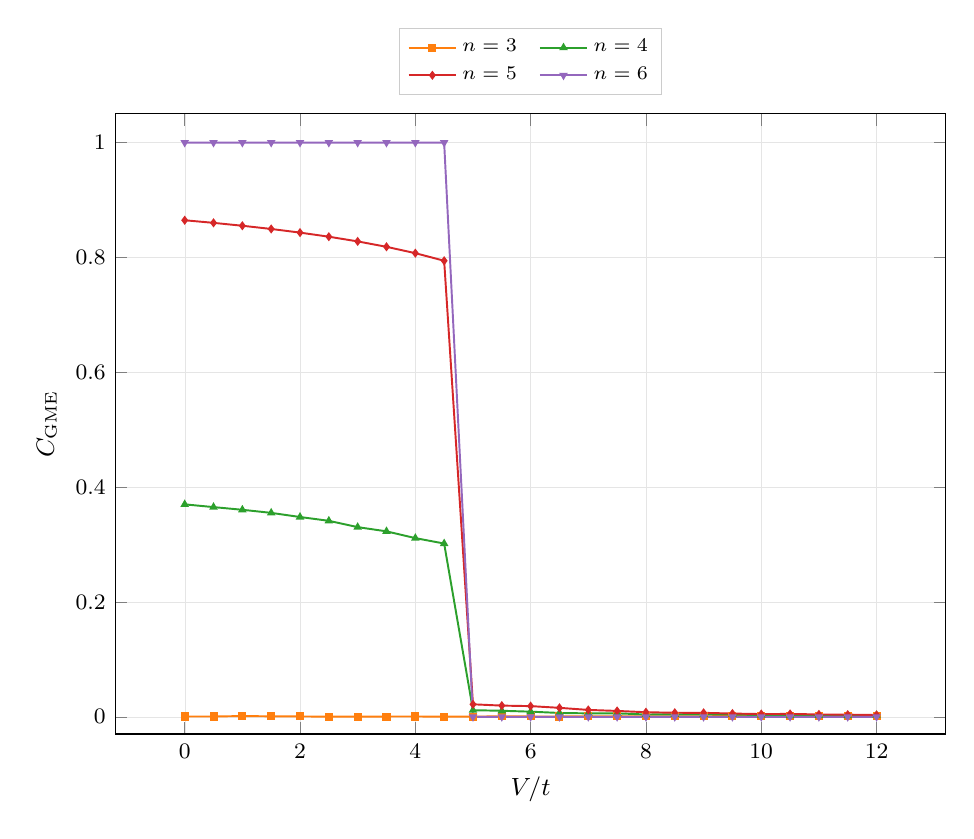
\begin{tikzpicture}
  \begin{axis}[
    width=\columnwidth,
    height=0.78\columnwidth,
    xlabel={$V/t$},
    ylabel={$C_{\mathrm{GME}}$},
    grid=both,
    grid style={line width=.1pt, draw=gray!20},
    tick label style={font=\footnotesize\rmfamily, /pgf/number format/fixed},
    label style={font=\small\rmfamily},
    scaled ticks=false,
    legend style={font=\scriptsize\rmfamily, draw=gray!40, at={(0.5,1.03)}, anchor=south, /tikz/every even column/.append style={column sep=6pt}},
    legend cell align={left},
    legend columns=2,
    ymin=-0.03,
    ymax=1.05,
  ]
    \addplot[color=gmeC1, mark=square*, mark size=1.1pt, line width=0.7pt] coordinates {
        (0,0.00053) (0.5,0.000519) (1,0.001334) (1.5,0.000794)
        (2,0.000601) (2.5,0.000297) (3,0.000471) (3.5,0.000475)
        (4,0.00055) (4.5,0.000282) (5,0.000442) (5.5,0.000761)
        (6,0.000589) (6.5,0.000553) (7,0.00089) (7.5,0.001041)
        (8,0.000967) (8.5,0.000929) (9,0.000911) (9.5,0.001293)
        (10,0.001115) (10.5,0.000789) (11,0.00133) (11.5,0.000842)
        (12,0.001277)
    };
    \addlegendentry{$n=3$}
    \addplot[color=gmeC2, mark=triangle*, mark size=1.1pt, line width=0.7pt] coordinates {
        (0,0.369961) (0.5,0.365182) (1,0.360514) (1.5,0.355157)
        (2,0.347936) (2.5,0.341299) (3,0.330316) (3.5,0.32297)
        (4,0.311175) (4.5,0.301738) (5,0.011513) (5.5,0.010511)
        (6,0.008951) (6.5,0.006715) (7,0.005979) (7.5,0.006051)
        (8,0.004002) (8.5,0.004354) (9,0.004) (9.5,0.004016)
        (10,0.003045) (10.5,0.002006) (11,0.002629) (11.5,0.002186)
        (12,0.002732)
    };
    \addlegendentry{$n=4$}
    \addplot[color=gmeC3, mark=diamond*, mark size=1.1pt, line width=0.7pt] coordinates {
        (0,0.864713) (0.5,0.860188) (1,0.855157) (1.5,0.849535)
        (2,0.843215) (2.5,0.836058) (3,0.827884) (3.5,0.818448)
        (4,0.807398) (4.5,0.794196) (5,0.021778) (5.5,0.019508)
        (6,0.018615) (6.5,0.015626) (7,0.011991) (7.5,0.010236)
        (8,0.008002) (8.5,0.007037) (9,0.00695) (9.5,0.005665)
        (10,0.004786) (10.5,0.005034) (11,0.004128) (11.5,0.003722)
        (12,0.003276)
    };
    \addlegendentry{$n=5$}
    \addplot[color=gmeC4, mark=triangle*, mark size=1.1pt, mark options={rotate=180}, line width=0.7pt] coordinates {
        (0,1) (0.5,1) (1,1) (1.5,1)
        (2,1) (2.5,1) (3,1) (3.5,1)
        (4,1) (4.5,1) (5,0) (5.5,0)
        (6,0) (6.5,0) (7,0) (7.5,0)
        (8,0) (8.5,0) (9,0) (9.5,0)
        (10,0) (10.5,0) (11,0) (11.5,0)
        (12,0)
    };
    \addlegendentry{$n=6$}
  \end{axis}
\end{tikzpicture}
